\documentclass[xcolor=dvipsnames]{beamer}
\usepackage{graphicx}
\usepackage{amsmath,amssymb}
\usepackage{multirow}
%\usepackage{mathtools}
\usepackage[ruled]{algorithm2e}


\usetheme{Madrid}

\newcommand*\oldmacro{}
%\newcommand{\longsearrow}{\lower 1.4ex\hbox{\begin{picture}(18,18)(0,0)
%\put(0,18){\vector(1,-1){18}}
%\end{picture}}}
\def\A{{\mathcal A}}
\def\B{{\mathcal B}}
\def\Q{{\mathcal Q}}

\def\b1{{\mathbf 1}}
\def\bone{{\mathbf 1}}
\def\b0{{\mathbf 0}}
\def\bb{{\mathbf b}}
\def\bx{{\mathbf x}}
\def\bw{{\mathbf w}}
\def\be{{\mathbf e}}
\def\bu{{\mathbf u}}
\def\bv{{\mathbf v}}
\def\br{{\mathbf r}}
\def\bg{{\mathbf g}}
\newcommand{\vc}{\boldsymbol}
\newcommand{\N}{{\mathcal N}}
\newcommand{\R}{{\mathcal R}}
\newcommand{\M}{{\mathcal M}}
\newcommand{\Range}{{\mathcal Range}}
\renewcommand{\Ref}[1]{\mbox{(\ref{#1})}}
%\DeclarePairedDelimiter\ceil{\lceil}{\rceil}

\newcommand{\e}{\varepsilon}
\newcommand{\RR}{\mathbb{R}}
\newcommand{\FF}{\mathbb{F}}
\newcommand{\CC}{\mathbb{C}}
\newcommand{\NN}{\mathbb{N}}
\newcommand{\ZZ}{\mathbb{Z}}
\newcommand{\QQ}{\mathbb{Q}}

\let\oldmacro\insertshorttitle% save previous definition
\renewcommand*\insertshorttitle{ILU0 / MDF for DG}
\usebeamertemplate{mytheme}

\renewcommand{\div}{\operatorname{div}}
\newcommand{\grad}{\operatorname{grad}}

\title{Adaptive Algebraic Multigrig Preconditionering}

\subtitle{with Graph Modularity Matching}

\author[Nelson/Vassilevski]{Austen Nelson \inst{1}  and Panayot S. Vassilevski\inst{1}}

%\vspace*{-0.05cm}

\institute[PSU]{\small
\vspace*{-0.2cm}
 \inst{1}
Portland State University,  ajn6@pdx.edu, panayot@pdx.edu
}

\vspace*{0.5cm}

\date[06-15-2023]
{{\color{blue} MTH 510 --- Multilevel Methods}\\ June 15, 2023}
\vspace*{-0.4cm}
\titlegraphic{\includegraphics[width=3.5cm,height=0.75cm]{PSU_logo.png}}

\begin{document}

\frame{\titlepage}
\begin{frame}
\frametitle{Overview}
\tableofcontents
%\tableofcontents[pausesections]
\end{frame}

\section{Background}
\subsection{Problem Statement}
\begin{frame}
  \frametitle{Problem Statement}
  Want to solve the linear matrix system:
  $$A \vc x = b$$

  Where $A$ is symmetric positive definite.

  A common source of problems like this is from numerical
  discretizations of elliptic partial differential equations:

  $$
  \begin{cases}
    -\Delta u = f &, \text{ in } \Omega\\ 
    u = 0 &, \text{ on } \partial \Omega
  \end{cases}
  $$

\end{frame}

\subsection{Algebraic vs Geometric Multigrid}
\begin{frame}
  \frametitle{Algebraic vs Geometric Multigrid}

  \textbf{Geometric Multigrid}
  \begin{itemize}
    \item Requires a hierarchy of refinements ($h$ or $p$)
    \item Interpolation and restriction operators come from this hierarchy
  \end{itemize}

  \textbf{Algebraic Multigrid}
  \begin{itemize}
    \item No knowledge of problem structure/nature required
    \item `Black Box' for the end user
    \item Takes a matrix and algebraically finds the interpolation and restriction operators
  \end{itemize}
\end{frame}

\subsection{Anisotropy}
\begin{frame}
  \frametitle{Anisotropy}
  
  Let $\Omega \subset \RR^3$.\\
  We can modify our original PDE to be of the form:
  $$
  \begin{cases}
    -\nabla \cdot (\beta \nabla u) = f &,\text{ on } \Omega\\ 
    u=0 &,\text{ on } \partial \Omega
  \end{cases}
  $$

  Where 
  $$\beta = \e I + \vc b \vc b^T$$
  for small $\e > 0$ and
  $$\vc b = \begin{bmatrix} \cos \theta \cos \phi\\ \sin \theta 
  \cos \phi \\ \sin \phi \end{bmatrix}$$

\end{frame}

\subsection{Heterogeneous Coefficients}
\begin{frame}
  \frametitle{Heterogeneous Coefficients}
  
  $$
  \begin{cases}
    -\nabla \cdot (\beta \nabla u) = f &,\text{ on } \Omega\\ 
    u=0 &,\text{ on } \partial \Omega
  \end{cases}
  $$

    \begin{center} 
      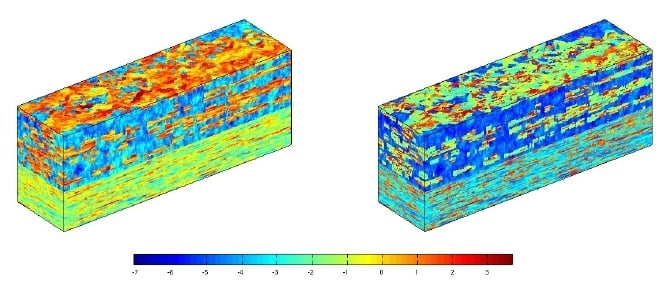
\includegraphics[width=\textwidth]{spe10perm.jpg}
    \end{center} 

\end{frame}

\section{Algorithm}
\begin{frame}
  \frametitle{Adaptivity Algorithm}
  Start with the `identity' preconditioner, $B = I$.
  \begin{itemize}
    \item Finding `Near Null' Vectors
      \begin{itemize}
        \item Search for an `algebraically smooth' error vector
          by iterating on the system $A \vc x = 0$ with a random
          starting guess with the preconditioner $B$.
        \item When the convergence stalls, $A \vc x \approx 0$
          and $\vc x$ is a linear combination of eigenvectors of 
          $A$ associated with small eigenvalues.
        \item If the test converged, i.e
          $$\frac{\|x\|_A}{\|x_{init}\|_A} < \e$$
          then return the current preconditioner $B$.
        \item Normalize this iterate to create the weight vector:
          $$\vc w = \frac{\vc x}{\|\vc x\|_A}$$
      \end{itemize}
    \item Construct the weighted matrix
      $\overline{A} = (\overline{a}_{ij})^n_{i,j=1}$ where
      $\overline{a}_{ij} = -w_i a_{ij} w_j$. Note that if
      $\vc w$ is `good enough' then $\overline{A}$ has positive
      row sums:
      $$r_i \equiv \sum_j \overline{a}_{ij} \approx a_{ii} w_i^2 \geq 0 \text{ since } a_{ii} > 0$$

  \end{itemize}

\end{frame}

\begin{frame}
  \frametitle{Adaptivity Algorithm}
  \begin{itemize}
    \item With positive row sums we can perform clustering of $A$
      through pairwise aggregation iterations on the modularity
      matrix, $B = (b_{ij})_{i,j=1}^n$, 
      associated with $\overline{A}$:

      Let $\vc r = (r_i)_{i=1}^n$ and $T = \sum_{i=1}^n r_i$.
      $$B = \overline{A} - \frac{1}{T} \vc r \vc r^T$$
    \item Performing these actions recursively gives a hierarchy
      aggregations, $\{P_k\}_{k=1}^\ell$, which in turn define a
      hierarchy of matrices, $\{A_k\}_{k=1}^{\ell+1}$:
      $$A_1 = A, \quad A_{k+1} = P_k^T A_k P_k $$
  \end{itemize}

\end{frame}

\begin{frame}
  \frametitle{Adaptivity Algorithm}
  \begin{itemize}
    \item Now we put $\vc w$ into the range of $P_1$,
      specifically such that $\vc w = P_1 \vc 1_2$. We
      do this by scaling row $i$ of $P_1$ by $w_i$.

    \item Using this modified hierarchy of aggregation operators
      and the resulting hierarchy of matrices we define an
      AMG V-cycle, denoted $B_{new}$.
    \item Create the composite preconditioner by composing
      $B$ with $B_{new}$ with the following algorithm:

      Initialize: $\vc x = 0$.
      \begin{itemize}
        \item $\vc x = \vc x + B \vc r$
        \item $\vc r = \vc r - A \vc x$
        \item $\vc x = \vc x + B_{new} \vc r$
        \item $\vc r = \vc r - A \vc x$
        \item $\vc x = \vc x + B \vc r$
      \end{itemize}
      Output $\vc x$.
    \item Define the new preconditioner, $B$ as the steps above.
    \item Return to the first step to search for new near null.
  \end{itemize}

\end{frame}

\section{Results}
\begin{frame}
  \frametitle{Results}
\end{frame}

\end{document}
